
%(BEGIN_QUESTION)
% Copyright 2008, Tony R. Kuphaldt, released under the Creative Commons Attribution License (v 1.0)
% This means you may do almost anything with this work of mine, so long as you give me proper credit

Two flowmeters are used to simultaneously measure the flow rate of a liquid through a pipe coming from a positive displacement pump:

$$\includegraphics[width=15.5cm]{i03634x01.eps}$$

Suppose the positive displacement pump continues to turn at a constant speed, with the temperature of the incoming liquid constant.  Suddenly, a steam pipe located near the pump breaks open, directing hot steam at the discharge pipe of the pump, heating the fluid as it exits the pump.

\vskip 10pt

Determine the effect this change in fluid discharge temperature will have on the output signals coming from both flowmeters (vortex and thermal), then explain your answer in detail.

\vfil 

\underbar{file i03634}
\eject
%(END_QUESTION)





%(BEGIN_ANSWER)

This is a graded question -- no answers or hints given!

%(END_ANSWER)





%(BEGIN_NOTES)

\begin{itemize}
\item{} Vortex flowmeter signal will {\bf increase}
\item{} Thermal (mass) flowmeter signal will {\bf remain the same}
\end{itemize}

The liquid density decrease resulting in the steam's heating of the fluid causes volumetric flow output from the pump to increase, while mass flow rate remains the same.  This will cause the vortex flowmeter to register a {\it greater} flow rate while the thermal (mass) flowmeter outputs the {\it same} signal it did before.  

Note that the accuracy of the flowmeters themselves will not be compromised by the increased temperature, but rather the actual volumetric versus mass flow rates of the fluid will change due to the increased temperature.

%INDEX% Measurement, flow: thermal (mass)
%INDEX% Measurement, flow: vortex

%(END_NOTES)


